\section{Miary ewaluacji}
W celu oceny skuteczności systemu detekcji wykorzystano następujących miary:
\begin{itemize}
    \item pole powierzchni pod krzywą Receiver Operating Characteristic (ROC) \\
    miara określa prawdopodobieństwo, że losowy element klasy pozytywnej(anomalii) otrzyma wyższą wartość anomalności niż losowo wybrany element klasy negatywnej (poprawna obserwacja). Krzywa ROC:
    \begin{figure}[!h]
        \centering
        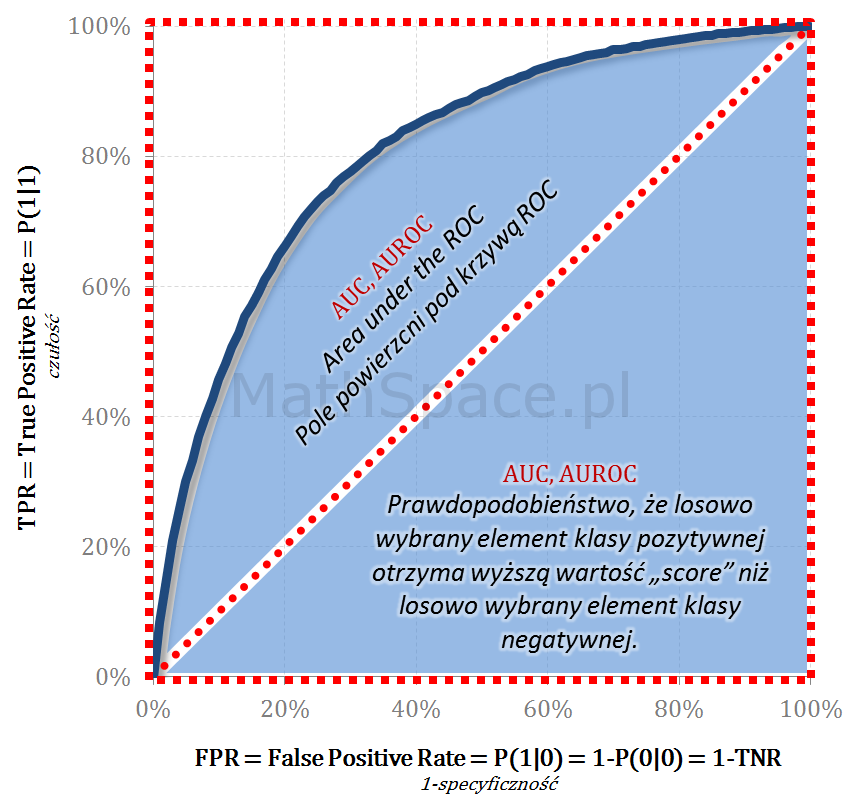
\includegraphics[width = 0.6\textwidth]{chapters/analiza/img/ROC-interpr-AUROC.png}
        \caption{Interpretacja pola pod krzywą ROC}
        \footnotesize{źródło: \cite{roc-image} }
        \label{fig:my_label}
    \end{figure}
    \item precyzja dla top n obserwacji (P@N) \\
    miara oblicza precyzję dla top n obserwacji, gdzie n oznaczać będzie sumę obserwacji odstających w zbiorze danych. Precyzja określa stosunek klasyfikacji prawdziwie pozytywnych (TP) do sumy klasyfikacji prawdziwie pozytywnych (TP) i fałszywie pozytywnych (FP):
    \begin{equation}
        precyzja = \frac{TP}{TP+FP}
    \end{equation}
\end{itemize}
Wykorzystane metryki wybrane były jako informatywny sposób oceny skuteczności detekcji anomalii \cite{campos2016evaluation}. Jak również wykorzystane były w benchmarku algorytmów zawartego w dokumentacji biblioteki PyOD.

\section{Wykorzystane zbiory danych }
Wykorzystano bazę zbiorów danych ODDS \cite{ODDS}. W celu ewaluacji wykorzystano zbiory danych, dla których w dokumentacji biblioteki PyOD przeprowadzono analizę skuteczności detekcji anomalii dla wybranych zbiorów danych.